%%%%%%%%%%%%%%%%%%%%%%%%%%%%%%%%%%%%%%%%%%%%%%%%%%%%%%%%%%%%%%%%%%%%%%%%
% Uni Duesseldorf
% Lehrstuhl fuer Datenbanken und Informationssysteme
% Vorlage fuer Bachelor-/Masterarbeiten
% Optimiert fuer den Original-Latex-Kompiler LATEX.EXE (LaTeX=>PS=>PDF)
%%%%%%%%%%%%%%%%%%%%%%%%%%%%%%%%%%%%%%%%%%%%%%%%%%%%%%%%%%%%%%%%%%%%%%%%
% Ueberarbeitung für pdflatex (LaTeX=>PDF)
%%%%%%%%%%%%%%%%%%%%%%%%%%%%%%%%%%%%%%%%%%%%%%%%%%%%%%%%%%%%%%%%%%%%%%%%
% Vorlage Changelog:
% 10.09.2015 (Matthias Liebeck): Nummerierung des Inhaltsverzeichnis nun römisch, Beispiel für einen Anhang eingebaut, \raggedbottom hinter sections eingefügt
% 11.07.2018 (Matthias Liebeck): Ersetzung des Bibliographiestils, Einsatz von Biber
% 04.09.2018 (Matthias Liebeck):
%   * Bibtex: unnötige Bibtexfelder beim Rendern ausblenden (thx @ Markus Brenneis)
%   * ngerman: "et al." im BibTeX für drei oder mehr Autoren
%   * Neuer Befehl \sectionforcestartright: Sections immer rechts beginnen (thx @ Philipp Grawe)
%   * ngerman: Deutsche Anführungszeichen im Literaturverzeichnis (thx @ Markus Brenneis)
%   * ngerman: Deutsche Anführungszeichen im Literaturverzeichnis (thx @ Markus Brenneis)
% 16.10.2018 (Matthias Liebeck): Zwei fixes an \sectionforcestartright (thx @ Markus Brenneis)
%%%%%%%%%%%%%%%%%%%%%%%%%%%%%%%%%%%%%%%%%%%%%%%%%%%%%%%%%%%%%%%%%%%%%%%%
%%%% BEGINN EINSTELLUNG FUER DIE ARBEIT. UNBEDINGT ERFORDERLICH! %%%%%%%
%%%%%%%%%%%%%%%%%%%%%%%%%%%%%%%%%%%%%%%%%%%%%%%%%%%%%%%%%%%%%%%%%%%%%%%%
% Geben Sie Ihren Namen hier an:
\newcommand{\bearbeiter}{Marvin Lindemann}

% Geben Sie hier den Titel Ihrer Arbeit an:
\newcommand{\titel}{Contig-Assembly der MHC-Region mittels Linearer Programmierung}

% Geben Sie das Datum des Beginns und Ende der Bachelorarbeit ein:
\newcommand{\beginndatum}{09. Juni 2019}
\newcommand{\abgabedatum}{09.~September~2019}

% Geben Sie die Namen des Erst- und Zweitgutachters an:
\newcommand{\erstgutachter}{Prof. Dr. Gunnar W. Klau}
\newcommand{\zweitgutachter}{Dr. Alexander Dilthey}

% Falls Sie die Arbeit zweiseitig ausdrucken wollen,
% benutzen Sie die folgende Zeile mit
% \AN fuer zweiseitigen Druck
% \AUS fuer einseitigen Druck
\newcommand{\zweiseitig}{\AUS}

% Falls Sections immer rechts beginnen sollen. Gerade für Masterarbeiten
% interessant. Bei kurzen Bachelorarbeiten eher weniger zu verwenden.
\newcommand{\sectionforcestartright}{\AUS}
%\newcommand{\sectionforcestartright}{\AN}

% Falls die Arbeit in englischer Sprache verfasst 
% werden soll, dann benutzen Sie die folgende Zeile mit
% englisch fuer englische Sprache
% deutsch fuer deutsche Sprache
\newcommand{\sprache}{deutsch}

% Hier wird eingestellt, ob es sich bei der Arbeit um eine Bachelor- 
% oder Masterarbeit handelt (unpassendes auskommentieren!):
\newcommand{\arbeit}{Bachelorarbeit}
%~ \newcommand{\arbeit}{Masterarbeit}

%%%%%%%%%%%%%%%%%%%%%%%%%%%%%%%%%%%%%%%%%%%%%%%%%%%%%%%%%%%%%%%%%%%%%%%%
%%%% ENDE EINSTELLUNGEN %%%%%%%%%%%%%%%%%%%%%%%%%%%%%%%%%%%%%%%%%%%%%%%%
%%%%%%%%%%%%%%%%%%%%%%%%%%%%%%%%%%%%%%%%%%%%%%%%%%%%%%%%%%%%%%%%%%%%%%%%

% Die folgende Zeile NICHT EDITIEREN oder loeschen
\input{titelmakros}

\pagenumbering{arabic}
\setcounter{page}{1}

%%%%%%%%%%%%%%%%%%%%%%%%%%%%%%%%%%%%%%%%%%%%%%%%%%%%%%%%%%%%%%%%%%%%%%%%
%%%% BEGINN TEXTTEIL %%%%%%%%%%%%%%%%%%%%%%%%%%%%%%%%%%%%%%%%%%%%%%%%%%%
%%%%%%%%%%%%%%%%%%%%%%%%%%%%%%%%%%%%%%%%%%%%%%%%%%%%%%%%%%%%%%%%%%%%%%%%

%%%%%%%%%%%%%%%%%%%%%%%%%%%%%%%%%%%%%%%%%%%%%%%%%%%%%%%%%%%%%%%%%%%%%%%%
% Text entweder direkt hier hinein schreiben oder, im Sinne der
% besseren Uebersichtlich- und Bearbeitbarkeit mittels \input die
% einzelnen Textteile hier einbinden.
%%%%%%%%%%%%%%%%%%%%%%%%%%%%%%%%%%%%%%%%%%%%%%%%%%%%%%%%%%%%%%%%%%%%%%%%
\section{Einleitung} \raggedbottom 
Der Major Histocompatibility Complex, kurz MHC, ist ein Teilstück der DNA von Wirbeltieren, welches unter anderem eine tragende Rolle bei Vorgängen des Immunsystems besitzt. Durch seine große Variabilität dient es als Ausweis der körpereigenen Zellen, um sich vor dem Immunsystem von Fremdgewebe zu unterscheiden. Unter anderem ergibt sich daraus ein großes Interesse für Organtransplantationen, die konkrete Sequenz der MHC-Region zu kennen. Ferner ist der MHC der Teil des Genoms, mit der größten Relevanz für Erbkrankheiten. 
Leider resultiert aus der großen Variabilität ein eben so großes Problem bei der Analyse dieses Aufbaus. Um dieses Problem zu verstehen, müssen wir erst verstehen, wie bei der Assemblierung, also der Bestimmung der DNA-Sequenz, vorgegangen wird.\\

Etablierte DNA-Sequenzierungstechnologien ermöglichen keine direkte Ermittlung der Basenpaare bei langen DNA-Sequenzen. Daher werden sie in kürzere Stücke zerlegt, für die dann die Basenpaare bestimmt werden können. Diese kürzere Stücke heißen \emph{Reads}. Für das Erstellen solcher Reads gibt es verschiedene Verfahren, die alle verschiedene Vor- und Nachteile haben. So werden bei der sogenannten Illumina-Sequenzierung sehr kleine Reads mit einer Länge von ungefähr 200 Basenpaaren erzeugt. Diese können sich teilweise überlappen, wodurch es möglich ist, einige Reads zu so genannten \emph{Contigs} zusammenzufügen. Im Idealfall passen die Reads so gut zueinander, dass der gesamte untersuchte DNA-Bereich rekonstruiert werden kann. Ein Fall, bei dem dies nicht möglich ist, zeigt diese Situation:
\begin{align*}
\text{ATTAAGCCTTAGGGTTATATCATATA}&\text{TATATATA}\\
&\text{TATATATATATGTAAGCGTTCGTTGTCTC}
\end{align*}
\begin{figure}[b]
\begin{center}
\includegraphics[width=0.9\textwidth]{bilder/repeat}
\end{center}
\caption{Repeat in einer Sequenz}
\label{repeat}
\end{figure}
Durch den sehr simplen Aufbau des Zwischenbereiches aus abwechselnden Adenin- und Thyminbasen ist es nicht möglich, die genaue Positionierung zu bestimmen. Auch wenn die Contigs nicht exakt zueinander positioniert werden können, so ist dies zumindest ungefähr möglich. Noch größere Schwierigkeiten machen Regionen in der DNA, die über eine längere Strecke komplett identisch sind, sogenannte Repeats. Das Problem wird in Abbilding \ref{repeat} verdeutlicht. Zu sehen sind fünf Contigs, wobei ein Pfeil von Contig $a$ zu Contig $b$ verdeutlicht, dass in der DNA Contig $a$ direkt vor Contig $b$ kommt. Da Contig 63 (blau) zwei mal in der DNA vorkommt, ist es nicht trivial zu bestimmen, wie der Strang verläuft. Und MHC ist sehr repetitiv, besitzt also viele Wiederholungen. Daher ist diese Methode ungeeignet um MHC zu assemblieren.


Eine weitere Möglichkeit der Sequenzierung ist die Nanopore-Sequenzierung. Hierbei können sehr lange Reads von über 10\,000 Basenpaaren gelesen werden. Aufgrund des Längenunterschieds werden die Reads aus der Illuminar Sequenzierung auch \emph{Short-Reads} genannt, und die Reads aus der Nanopore-Sequenzierung \emph{Long-Reads}. Durch ihre Länge umfassen die Long-Reads oftmals bereits vollständige Repeats plus Umgebung. In unserer Abbildung entspräche dies einem Read, in dem Contig 132, Contig 63 und Contig 32 (gelb, blau und grün) Teil von einem Read sind und es keine Schwierigkeiten diesbezüglich gibt. Leider ist die Fehlerrate bei dieser Methode sehr hoch. 
So werden sehr viele Long-Reads aus der selben Region benötigt, um die richtigen Basenpaare verlässlich zu bestimmen.


Daher hat sich die Manchot-Forschungsgruppe vom Institut für Medizinische Mikrobiologie und Krankenhaushygiene der HHU, mit deren Zusammenarbeit diese Arbeit entstand, eine Kombination der beiden Methoden entwickelt.
% Diese deren Nachteile ausgleichen soll. 
Die verlässlichen Contigs aus der Illuminar-Sequenzierung wurden auf die Long-Reads gemappt und so deren Abstände zueinander bestimmt. Betrachten wir zur Anschauung Abbildung \ref{longread} eines Long-Reads. Die kleinen rot eingefärbten Bereiche stellen Fehler dar, die bunten Bereiche stellen Gebiete dar, in denen die Basenpaarsequenzen mit denen eines Contigs aus den Illuminar-Daten übereinstimmen. In der selben Situation wie in Abbildung \ref{repeat} hätten wir nun die Information erhalten, dass Contig 114 und Contig 32 zusammengehören, also die rechte Auflösung der Abbildung richtig ist. 
\begin{figure}
\begin{center}
\includegraphics[width=0.8\textwidth]{bilder/longread}
\end{center}
\caption{Ein Long-Read über mehrere Contigs}
\label{longread}
\end{figure}
Die Manchot-Forschungsgruppe hat diese Daten gesammelt und daraus eine Liste aus paarweisen Daten extrahiert. Diese besitzt die Form: Contig $a$ hat zu Contig $b$ die Entfernung $d$ (in Anzahl von Basenpaaren zwischen $a$ und $b$). Dieses Dreiertuple aus zwei Contigs und einer Distanz nennen wir einen \emph{Constraint}.


Es bleiben noch einige Schwierigkeiten für die Assemblierung zu beachten. Die Distanzwerte zwischen den Contigs sind meistens durch Fehler in den Long-Reads verfälscht. Dadurch sind erst mehrere Constraints, die eine ähnliche Distanz zwischen zwei Contigs prognostizieren, wirklich belastend. Bis zu welchen Distanz sich Constraints noch bestätigen und ab wann sie sich widersprechen ist hierbei ein entscheidender Aspekt, der betrachtet werden muss. Die Repeats lassen sich nicht immer so eindeutig auflösen wie in unserem Beispiel. In manchen Fällen kann erst im Gesamtzusammenhang erkannt werden, wie der Strang verläuft. Letztlich bleibt noch die große Datenfülle als Herausforderung zu nennen: Bei rund 122\,000 auftretenden Distanzen zwischen 2\,124 Contigs ist eine manuelle Zusammenfügung nicht zielführend und mindestens eine Teilautomatisierung der Prozesse obligatorisch. Auf der anderen Seite sind die Constraints nicht gleichmäßg verteilt, sodass es Regionen gibt, bei denen mit sehr wenig Informationen ausgekommen werden muss.

Hier stellt sich die Frage, mit welchen Methoden diese Probleme bewältigt werden können. Denkbar wäre eine Umsetzung mittels Linearer Programmierung. Das Ziel dieser Arbeit wird sein, zu untersuchen, ob lineare Programmierung hierbei anwendbar ist, und welche Vor- und Nachteile lineare Programme mit sich bringen.


\section{Formalisierung}\raggedbottom 

Die vorliegenden Daten der Manchot-Forschungsgruppe bestehen aus zwei Dateien: 
\begin{enumerate}
\item einer Liste von allen Contigs und deren Länge gemessen in der Anzahl an Basenpaaren, die im Contig auftreten
\item einer Datei mit den eingangserwähnten Constraints.
\end{enumerate}
Letztere besitzt folgenden dreispaltigen Aufbau:
\begin{align*}
&a \quad b \quad 1000\\
&a \quad b \quad 1100\\
&b \quad c \quad 3000\\
&a \quad c \quad 6000
\end{align*}
Dabei entspricht jede Zeile einem Constraint. Die ersten beiden Zeilen geben jeweils die beiden involvierten Contigs an. In der dritten Spalte sind die gemessenen Distanzen angegeben. Diese sind als Entfernung vom rechten Rand des ersten Contigs zum linken Rand des zweiten Contigs in Basenpaaren zu interpretieren. Negative Distanzen sind auf Überlagerungen einzelner Contigs zurückzuführen. Zusätzlich zu den Constraints aus den Long-Reads stammen etwa 2\% der Constraints direkt aus der Illumina Sequenzierung. Hier wurde mehrmals die Distanz zwischen benachbarte Contigs gemessen und der Durchschnitt daraus berechnet. Dadurch können auch nicht ganzzahlige Werte als Distanzen auftreten.

\subsection{Anforderungen an die Lösung}
Nun wollen wir einige Gütekriterien für mögliche Lösungen festlegen, um während der Bearbeitung Orientierungspunkte für die weitere Optimierung des Algorithmus zu haben und um diesen nach Abschluss anhand dieser Kriterien zu bewerten.
Folgende Punkte sollen beachtet werden:
\begin{enumerate}
\item Wenn mehrere Constraints eine ähnliche Distanz zwischen zwei Contigs sehen, sollten diese Contigs auch die Distanz möglichst gut erfüllen. Der Schwellwert hierbei liegt bei zwei Constraints.
\item Ein Großteil der restlichen Constraints sollte auch zu der Positionierung passen.
\item Es sollten möglichst wenig Contigs nahe zueinander positioniert werden, die keine gemeinsamen Constraints aufweisen. Diese Situation wird durch Abbildung \ref{gespallten} illustriert. In der Abbildung werden die Constraints durch gerichtete Kanten zwischen den Contigs dargestellt. Der oberer Teilabschnitt zeigt eine Lösung, bei der die Bedingung nicht erfüllt wurde. Realistischer ist jedoch, dass hierbei ein Teilblock bestehend aus Contig 12 und Contig 32 doppelt in dem DNA-Strang vorkommt und bei der Lösung des Problems zwei separate Stränge ineinander verflochten wurden. Dies ist in der unteren Bildhälfte dargestellt.

\begin{figure}
	\begin{center}
		\includegraphics[width=1\textwidth]{bilder/gespallten}
	\end{center}
	\caption{verflochtene Stränge}
	\label{gespallten}
\end{figure}
	
\item Die Entfernung vom ersten zum letzten Contig sollte zwischen 4,8 Millionen und 5 Millionen Basenpaare lang sein, da dies die ungefähre Gesamtlänge des Strangs ist.
\item Bei einer Lösung wäre es zudem gut, wenn man Informationen darüber besitzen würde, wie wahrscheinlich es ist, ob verschiedene Teilgebiete tatsächlich so im Strang auftreten. Dabei wäre zum Beispiel eine Unterteilung in „sichere“ und „unsichere“ Gebiete interessant.
\end{enumerate}

Nun wollen wir konkretisieren, bis zu welchem Abstand Constraints ähnliche Distanzen haben. Dazu betrachten wir, wie die Standardabweichung der Distanzen von Constraints verteilt ist.
In der Abbildung \ref{std} werden die zu einem Basenpaar zugehörigen Constraints gegen ihre Standardabweichung geplottet. 
Dabei wurden pro Basenpaar die jeweiligen Distanzen der Constraints zu einer (Multi-)Menge zusammengefasst. Es wurde symmetrisch vorgegangen, das heißt Paare der Form (a,b) und (b,a) werden in der gleichen Menge behandelt. Ferner wurden Mengen mit einem Element nicht berücksichtigt, da es hier keine Abweichung gibt. Für die jeweiligen Mengen wurden dann die Standardabweichungen berechnet, der Größe nach geordnet und dann mit Berücksichtigung dieser Ordnung geplottet.
Der Plot wird mit zwei Skalierungen angegeben: Auf der linken Seite sieht man eine logarithmische Skalierung, während der rechte Plot eine lineare Skalierung verwendet.

\begin{figure}
	\begin{center}
		\includegraphics[width=0.8\textwidth]{bilder/std}
	\end{center}
	\caption{Standardabweichung der Distanzwerte}
	\label{std}
\end{figure}




Eine optische Betrachtung der Plots legt folgende Interpretation nahe: 
Es gibt einen Bereich der natürlichen Abweichung in der Datenmenge. Dies entspricht dem relativ flachen Anfangsbereich des Graphen. Ab einem gewissen Punkt "explodieren" die Werte. Hier ist die Standardabweichung innerhalb der Constraints so hoch, dass man nicht mehr von natürlicher Abweichung innerhalb der Daten ausgehen kann. Die orangene Linie grenzt diese Bereiche intuitiv voneinander ab. 
Diese liegt bei einer Standardabweichung von 500 Basenpaaren. 
Somit unterstützen sich Constraints, deren Distanzwerte sich nicht um mehr als 500 Basenpaare unterscheiden.

Um die oben genannten Forderungen an eine Lösung zu erfüllen, ist es notwendig die Repeats auszumachen und die Constraints auf diese Repeats aufzuteilen. Dazu halten wir uns an das Prinzip: $\glqq$so viel wie nötig, so wenig wie möglich$\grqq$.
Um dies sicherzustellen, sollte ein Contig, der mehrfach in der DNA vorkommen soll, zwei Punkte für jede seiner Versionen erfüllen:

\begin{enumerate}
\item Es sollte mindestens ein Contig in der Nachbarschaft liegen, zu welchem es zwei oder mehr Constraints gibt.
\item Sowohl unter den Vorgängern als auch unter den Nachfolgern des Contigs, sollte es je einen Contig geben, der einen gemeinsamen Constraint aufweist.
\item Sowohl zu einem der Vorgängern als auch zu einem der Nachfolgern des Contigs, sollte es ein Constraint mit dem Contig geben.
\end{enumerate}
Der erste Punkt soll sicherstellen, dass es nicht einfach ein Fehler in den Daten ist. Der zweite Punkt stellt sicher, dass der richtige Contig als Repeat markiert wurde. Wenn der Distanzwert eines Constraints nicht erfüllt ist, ist erstmal nicht klar, welcher der beiden beteiligten Contigs eine Repeat-Version haben soll.

 % Gebiete anders zueinander stehen, als sie es gerade tun, so ist nicht klar welche der beiden Gebiete ein Repeat besitzt. Daher ist es Sinnvoll dass die Repeatversion Constraints zu beiden Seiten haben muss, um sich in den Strang zu integrieren.
%Denn wenn viele Constraints zwischen zwei Gebiete nahlegen, dass diese Gebiete anders zueinander stehen, als sie es gerade tun, so ist nicht klar welche der beiden Gebiete ein Repeat besitzt. Daher ist es Sinnvoll dass die Repeatversion Constraints zu beiden Seiten haben muss, um sich in den Strang zu integrieren.
\section{Das lineare Programm}
\subsection{Eine kurze Einführung}
Die Problemstellung in dieser Arbeit lässt sich als lineares Programm (kurz LP) formulieren. In der linearen Programmierung möchten wir, unter Berücksichtigung von linearen Nebenbedingungen an die Funktionsparameter, eine lineare Funktion maximieren oder minimieren.
Formal mathematisch lässt sich der Minimierungsfall so fassen:
\begin{align*}
	Gegeben:&\quad c \in \mathbb{R}^{n},\ A \in \mathbb{R}^{n \times m},\ b \in \mathbb{R}^{m} \\
	Gesucht:&\quad \argmin_{ x\in \mathbb{R}^n}\{c^Tx\,|\, Ax \leq b\}
\end{align*}
Dabei wird folgende Notation verwendet:
\begin{description}
\item[\quad Variablen] $x_1,..., x_n$
\item[\quad Zielfunktion]  $c^Tx = \sum_{i=1}^n c_i x_i$
\item[\quad Nebenbedingungen]  $Ax \leq b \ \Leftrightarrow\ \sum_{i=1}^n a_{ji} x_i \leq b_j, \ j = 1,...,n$
\end{description}
Lineare Programme lassen sich in Polynomialzeit berechnen. Daher eignen sie sich oft als Werkzeug für verschiedenste Probleme. Es ist auch möglich, den Definitionsraum der Variablen (teilweise) auf ganze Zahlen zu beschränken. Dies bezeichnet man dann als ein ganzahliges lineares Programm (kurz ILP). ILPs bieten einige Möglichkeiten die mit LPs nicht umzusetzen wären. Sie sind dafür aber NP-schwer und somit wahrscheinlich nicht polynomialzeitberechenbar.

\subsection{Assembly als LP}
Im Folgenden bezeichnet $C$ die Menge aller Contigs und $D$ die Multimenge aller Constraints. Dabei wurde der Distanzwert jedes Constraints in $D$ so umgerechnet, dass er die Entfernung von linken Rand vom ersten Contig bis zum linken Rand des zweiten Contigs angibt.
Wir möchten die Contigs so positionieren, dass der durchschnittliche Fehler aller Constraints möglich klein ist. Als Formel:
\[ \pos = \argmin_{\pos\,:\, C \rightarrow \mathbb{N}} \ \sum_{(a,b,\delta) \in D} |\pos(b) - \pos(a) - \delta| \] 
Um daraus ein lineares Programm zu machen, führen wir für jeden Constraint $(a,b,\delta)$ aus $D$ eine Hilfsvariable $\varepsilon$ ein:
\[ \varepsilon = |\pos(b) - \pos(a) - \delta| \]
Mit Hilfe dieser Variablen können wir die zu minimierende Zielfunktion wie folgt darstellen:
\begin{align*}
\quad& \sum_{d \in D} \varepsilon_{d}
\end{align*}
Nun müssen wir noch die Informationen über die Fehler, also $\varepsilon = |\pos(b) - \pos(a) - \delta|$, einbauen. Da wir ohnehin die Summe der Fehler minimieren wollen, ist es ausreichend, folgende Ungleichung zu fordern:
\begin{align*}
\varepsilon \geq |\pos(b) &- \pos(a) - \delta|
\end{align*}
Dies liegt daran, dass bei Minimierung immer die untere Schranke angenommen wird, welche in diesem Fall die Gleichheit ist. Nun ist die Betragsfunktion aber nicht linear. Sie lässt sich aber äquivalent durch die folgenden beiden linearen Ungleichung darstellen:
\begin{align*}
\pos(b) - \pos(a) - \delta &\leq \varepsilon\\
-\pos(b) + \pos(a) + \delta &\leq \varepsilon
\end{align*}

Zusammengefasst erhalten wir also folgendes lineares Programm für die Berechnung der optimalen Positionierung:

\begin{align*}
\text{Variablen:}\quad& \pos(c) \ \forall c \in C \ \ \text{und} \ \ \varepsilon_{d} \ \forall \ d \in D\\
\text{Zielfunktion:}\quad& \sum_{d \in D} \varepsilon_{d}\\
\text{Bedingungen:}\quad \begin{split} \pos(b) - \pos(a) - \delta \leq \varepsilon_{d}\\
-\pos(b) + \pos(a) + \delta \leq \varepsilon_{d} \end{split}\quad \forall \ (a,b,\delta) = d \in D
\end{align*}
Distanzwerte weisen zu große Schwankungen auf, um auf ein Basenpaar genau zu sein. Daher bietet es sich an, die Relaxierung des LPs zu betrachten, also auch reelle Positionen zuzulassen. Durch diese Lockerung der Bedingungen lässt sich das Programm wesentlich schneller lösen.

Dieses LP sorgt nur dafür, dass die Constraints möglichst gut erfüllt sind. Weder verhindert es, dass Contigs, welche keine Constraints vorweisen, nahe positioniert werden, noch erkennt es Repeats. Um das weitere Vorgehen planen zu können, bietet es sich trotzdem an, diesen Ansatz auszuführen und anhand der Lösung konkrete Problemstellen zu lokalisieren. 


Die Implementierung erfolgt in der Jupyter-Umgebung der Programmiersprache Python. Dabei wird Gurobi, einem Programm das auf mathematische Optimierung spezialisiert ist, verwendet. Das Programm liefert uns als Rückgabe eine konkrete Positionierung der Contigs. Nun wäre es gut, wenn wir eine Möglichkeit hätten, festzustellen, inwiefern die von uns festgelegten Kriterien erfüllt sind. Im nächsten Kapitel werden dazu verschiedene optische Verfahren diskutiert

%Somit lässt es sich nur unterstützend einsetzen. Wie mit Hilfe von ILPs auch diese beiden Punkte abgedeckt werden könnten, diskutieren wir im letzten Kapitel.



\section{Wie man eine Lösung grafisch darstellt}
Ein wichtiger Aspekt für die Arbeit mit großen Datenmengen ist die Visualisierung.
Sie sollte in der Lage sein, die wichtigsten Informationen auf einen Blick sichtbar zu machen. Wir beschäftigen uns nun mit Möglichkeiten, konkrete Positionierungen der Contigs, also Abbildungen $pos: C \rightarrow \mathbb{R}$, zu visualisieren.
Eine erste, naheliegende Option ist eine lineare Darstellungsweise. Hierbei werden die einzelnen Contigs gemäß ihrer Positionierung und ihrer Länge auf der reellen Zahlengerade eingezeichnet. Um Überlappungen zu beachten, bietet es sich an, mehrschichtig zu arbeiten. Mehrschichtig bedeutet hier, dass bei Überlappung zweier Contigs der hintere Contig in einer anderen Höhe geplottet wird. Diese Methode wird durch Abbildung \ref{plotmehrschichtig} illustriert.
Vorteile dieser Darstellungsweise sind unter anderem die folgenden Aspekte:
\begin{enumerate}
\item Der gesamte Strang inklusive seiner Länge ist auf einen Blick sichtbar. Dies liefert dem Betrachter einen groben Überblick. Ferner lässt sich der fünfte Unterpunkt der Anforderungen an Lösungen, die Länge des Stranges, so auch optisch leicht überprüfen.
%\item Durch das mehrschichtige Arbeiten lassen sich Regionen mit einer hoher Überlappungsdichte (also hoher Coverage) leicht lokalisieren.
\item Regionen, die hauptsächlich aus großen oder aus kleinen Contigs bestehen, lassen sich anhand des Plots leicht lokalisieren. Für den fünften Unterpunkt unsere Anforderungen an eine Lösung lässt sich dies als Indiz für die Sicherheit dieser Umgebungen verwenden. In Gebieten, in denen nur wenige, aber große Contigs vorkommen, sollten im Schnitt weniger Fehler hinsichtlich der geringeren Datenmenge auftreten als in mit vielen kleinen Contigs überfüllten Regionen.
\item Durch Hinzunahme von Färbungen ist es möglich, einige Kerninformationen leicht zugänglich zu machen. Dazu zählen etwa die Anzahl der Repeats eines einzelnen Contigs oder der Gesamtanteil an sich wiederholenden Contigs.
\end{enumerate}
Jedoch gibt es einen zentralen Nachteil bei der Wahl dieser linearen Darstellungsform: Die Information, die wir durch die Constraints erhalten, werden in der Visualisierung nicht berücksichtigt.
Damit lässt sich die Einhaltung der ersten drei Kriterien an eine Lösung optisch nicht analysieren.
Beispielsweise sieht man nicht, ob benachbarte Contigs auch tatsächlich gemeinsame Constraints aufweisen.
Um auch die Constraints mit einzubeziehen, bedarf es einer weiteren Darstellungsweise.

Um auch die Constraints mit einzubeziehen, bedarf es einer weiteren Darstellungsweise.
Ähnlich wie in Abbildungen \ref{abb1} und \ref{abb3} lassen sich dafür gerichtete Graphen verwenden. Dabei bildet die Menge der Contigs die Knoten des Graphen. Constraints zwischen zwei Knoten lassen sich als (gerichtete) Kanten darstellen.
Um eine gewisse Übersichtlichkeit zu erhalten, ist es aber sinnvoll, nicht alle Constraints zu plotten.
Stattdessen nutzen wir die gegebene Positionierung aus und zeichnen nur Kanten für nah beieinander positionierte Contigs mit gemeinsamen Constraints.
Dabei gehen wir für jeden auftretenden Contig $a$ wie folgt vor:
\begin{itemize}
\item Zunächst werden alle Constraints gelöscht, deren Fehler in der vorgegebenen Positionierung größer als eine fixierte Konstante ist. Oftmals fällt die Wahl hier auf eine Zahl in der Größenordnung $500$ gemäß der Überlegungen bezüglich der Standardabweichungen in dem Kapitel der Formalisierung.
\item Ferner werden mehrfach auftretende Constraints zusammengefasst und alle Schleifen, also alle Constraints der Form $(a, a, d)$ gelöscht.
\item Sei nun $N_a$ die Menge aller Contigs, die zusammen mit $a$ in einem verbliebenden Constraints enthalten sind. Nun werden die Contigs in $N_a$ und $a$ selbst bezüglich ihrer Positionierung sortiert.
\item Schließlich wird je eine Kante von $a$ zu den ersten beiden Contigs, die hinter $a$ positioniert wurden, gezeichnet. Umgekehrt wird je eine Kante von den ersten beiden Contigs, die vor $a$ positioniert wurden, zu $a$ gezeichnet.
\end{itemize}
Im Allgemeinen tritt hierbei auch der Fall auf, dass eine Kante $(a,b)$ während des Prozesses doppelt eingezeichnet werden soll: Einmal im Durchgang von $a$ als auslaufende Kante und einmal im Durchgang von $b$ als einlaufende Kante.
Sie werden trotzdem nur einmal gezeichnet.

Die Wahl, dass jeder Knoten zwei Vorgänger und zwei Nachfolger bekommt, ist nicht fest, hat sich aber als besonders geeignet herausgestellt. Bei nur einem Vorgänger und einem Nachfolger kann es schnell passieren, dass ein eigentlich zusammenhängender Strang unzusammenhängend dargestellt wird. Abbildungen \ref{t} und \ref{tt} illustrieren diese Situation. Dabei entspricht die erste Abbildung der tatsächlich im Programm auftretenden Darstellungsform. In der zweiten Abbildung wurde die Situation noch einmal etwas schematischer skizziert und optisch mit Farben unterlegt. 
Auch können mehrere Kanten interessante Einblicke über die Struktur geben. So gibt es Contigs die nur eine einlaufende Kante besitzen, oder deren Kanten mehrere Contigs überspringen. Alles ein Zeichen von Unstimmigkeiten, die näher untersucht werden könnten.



%\begin{minipage}{0.5\textwidth}
%\begin{figure}
%	\begin{center}
%		\includegraphics[width=0.9\textwidth]{bilder/t}
%	\end{center}
%	\caption{t}
%	\label{t}
%\end{figure}
%\end{minipage}

%\begin{minipage}{0.5\textwidth}
%\begin{figure}
%	\begin{center}
%		\includegraphics[width=0.9\textwidth]{bilder/tt}
%	\end{center}
%	\caption{tt}
%	\label{tt}
%\end{figure}
%\end{minipage}
\section{Algorithmus Phase 1: Grobe Lösung aufbauen}
Wenn Gurken hinter Gurken gurken, gurken Gurken Gurken nach.\\
Hier fehlt Bild + Analyse + tolle Einleitung + Überleitung.

Wir benötigen ein Grundgerust, [...]

Dafür speichern wir die Constraints als einen gerichteten Multigraphen aus der NetworkX Bibliothek \ref{}, also für jeden Constraint $(a,b,d)$ eine Kante von $a$ nach $b$ der Länge $d$.

Für Zeitintensivere Berechnungen, erstellen wir eine reduzierte Version, in der ähnliche Kanten zusammengefasst werden zu einer Kante. Dabei werden für je zwei Contigs alle Distanzwerte zwischen diesen beiden Contigs sortiert (wobei für eine Richtung die Distanzwerte als negativ betrachtet werden). Dann werden die Distanzwerte aufgeteilt, sobald sie sich mehr als 500 Basenpaare zum nächsten Wert unterscheiden. Die so gruppierten Werte werden durch ihr Median ersetzt und mit der Gruppengröße Gewichtet. 

Gehen wir dies an einen kleinen Beispiel durch. Gegeben sind folgende Constraints zwischen zwei Contigs $a$ und $b$:
\begin{center}
\begin{tabular}{lr}
$a$\quad $b$\quad &100\\
$a$\quad $b$\quad &11\,000\\
$b$\quad $a$\quad &50\\
$b$\quad $a$\quad &60\,000\\
$a$\quad $b$\quad &70\\
$a$\quad $b$\quad &300\\
$a$\quad $b$\quad &10\,950\\
$a$\quad $b$\quad &11\,050\\
$a$\quad $b$\quad &20\\
$a$\quad $b$\quad &600\\
$b$\quad $a$\quad &200
\end{tabular}
\end{center}
Die sortierten Distanzwerte:
\[-60000\ \ \,{-200}\ \ \,{-50}\ \ \,20\ \ \,70\ \ \,100\ \ \,300\ \ \,600\ \ \,10950\ \ \,11000\ \ \,11050\]
Gruppen bilden bei Abständen über 500:
\[-60000\,|\, {-200}\ \ \,{-50}\ \ \,20\ \ \,70\ \ \,100\ \ \,300\ \ \,600\, |\, 10950\ \ \,11000\ \ \,11050\]
Es resultieren diese drei Kanten im reduzierten Graphen:

\begin{center}
\includegraphics[width=0.4\textwidth]{bilder/dreikannten}
\end{center}


Unser Ziel ist es, ein Pfad durch den den Graphen zu finden vom ersten bis zum letzten Contig, der möglichst viele Contigs beinhaltet.
Dafür werden wir beim ersten Contig anfangen und uns Schrittweise vorarbeiten. Sollte sich der Graph aufteilen, so versuchen wir zuerst mithilfe von Heuristiken zu bestimmen, welcher Pfad der richtige ist. Sollte dies nicht möglich sein, werden alle Pfade ausprobiert.

Wir beginnen mit Contig 2345APD an Position 0. Für jede auslaufende Kante $e$ aus 2345APD wird zu dem Endknoten von $e$ die Länge der Kante in einer Liste gespeichert. Die ersten Listen der ersten 10 Contigs sehen so aus:
\begin{footnotesize}
\begin{align*}
\text{1483APD}&: 6632\ \ \,6662\ \ \,6662\\
\text{1395APD}&: 6877\ \ \,6943\ \ \,6977\ \ \,6979\ \ \,6980\ \ \,6982\ \ \,6985\ \ \,6993\ \ \,6998\ \ \,6999\ \ \,7002\\
\text{1596APD}&: 9809\ \ \,9867\ \ \,9903\ \ \,9931\ \ \,9939\ \ \,9942\ \ \,9951\ \ \,9978\\
\text{2235APD}&: 14013\ \ \,14070\ \ \,14179\ \ \,14219\ \ \,14263\ \ \,14290\ \ \,14304\\
\text{1534APD}&: 14687\ \ \,14732\ \ \,14841\ \ \,14930\ \ \,14957\ \ \,14972\\
\text{546APD}&: 16242\ \ \,16254\ \ \,16372\ \ \,16470\ \ \,16550\\
\text{577APD}&: 18659\ \ \,18782\ \ \,18967\ \ \,19040\ \ \,19081\\
\text{998APD}&: 32244\ \ \,32453\\
\text{209APD}&: 34061\ \ \,34257\\
\text{1635APD}&: 43666
\end{align*}
\end{footnotesize}
Es folgen noch 101 weitere Contigs mit jeweils nur einen Eintrag. Diese Werte werden genau wie beim reduzierten Graphen gruppiert und der Contig mit der kleinsten Position wird als nächstes gesetzt. 

Dies ist in diesem Fall Contig 1483APD an Position 6662. Auch von 1483APD werden die Distanzwerte der auslaufenden Kannten genommen. Diese werden aber zuerst zu seiner Position addiert und dann zu den schon bestehenden Werten von 2345APD hinzugefügt:

\begin{footnotesize}
\begin{align*}
\text{1395APD:}&\ 6877\ \ \,6943\ \ \,6977\ \ \,6979\ \ \,6980\ \ \,6982\ \ \,6985\ \ \,6993\ \ \,6998\ \ \,6999\ \ \,7002\quad\quad 6982\ \ \, 6989\ \ \,6994\\
\text{1596APD:}&\ 9809\ \ \,9867\ \ \,9903\ \ \,9931\ \ \,9939\ \ \,9942\ \ \,9951\ \ \,9978\quad\quad 9906\ \ \,9946\\
\text{2235APD:}&\ 14013\ \ \,14070\ \ \,14179\ \ \,14219\ \ \,14263\ \ \,14290\ \ \,14304\quad\quad 14109\ \ \,14308\\
\text{1534APD:}&\ 14687\ \ \,14732\ \ \,14841\ \ \,14930\ \ \,14957\ \ \,14972\quad\quad 14771\ \ \,14976\\
\text{546APD:}&\ 16242\ \ \,16254\ \ \,16372\ \ \,16470\ \ \,16550\quad\quad 16293\ \ \,16554\\
\text{577APD:}&\ 18659\ \ \,18782\ \ \,18967\ \ \,19040\ \ \,19081\quad\quad 18698\ \ \,19044\\
\text{998APD:}&\ 32244\ \ \,32453\quad\quad 32248\\
\text{209APD:}&\ 34061\ \ \,34257\quad\quad 34065\\
\text{1635APD:}&\ 43666
\end{align*}
\end{footnotesize}
\section{Algorithmus Phase 2: Lösung mithilfe vom LP verfeinern}
\section{Auswertung der Ergebnisse}
\section{Diskussion}
%%%%%%%%%%%%%%%%%%%%%%%%%%%%%%%%%%%%%%%%%%%%%%%%%%%%%%%%%%%%%%%%%%%%%%%%
%%%% ENDE TEXTTEIL %%%%%%%%%%%%%%%%%%%%%%%%%%%%%%%%%%%%%%%%%%%%%%%%%%%%%
%%%%%%%%%%%%%%%%%%%%%%%%%%%%%%%%%%%%%%%%%%%%%%%%%%%%%%%%%%%%%%%%%%%%%%%%
\clearpage
% Entfernen Sie das Kommentar aus der nachfolgenden Zeile, falls Sie einen Anhang in der Arbeit verwenden wollen. Beachten Sie, dass Sie sich im Verlauf der Arbeit mit \ref{...} (z.B. \ref{anhang:zusatz1}) auf den Anhang beziehen.
%\input{anhang}
%\bibliography{references}
%\bibliographystyle{alphadin}
\DeclareNameAlias{sortname}{first-last}
\printbibliography[heading=bibintoc, title=References]
%\vspace*{\fill}
\clearpage
\listoffigures
\listoftables
%\pagebreak
%\printindex
\end{document}